%!TEX root = ../thesis.tex
%*******************************************************************************
%*********************************** First Chapter *****************************
%*******************************************************************************

\chapter{Introduction}  %Title of the First Chapter

\ifpdf
    \graphicspath{{Introduction/Figs/Raster/}{Introduction/Figs/PDF/}{Introduction/Figs/}}
\else
    \graphicspath{{Introduction/Figs/Vector/}{Introduction/Figs/}}
\fi
%********Literature Review************
%********Review HGSOC, microenvironments, spatial analysis, collagen, hypoxia, immune system and functionality/interactions************


%********************************** %First Section  **************************************
\section{What is Ovarian cancer?} %Section - 1.1 

Introduction to the thesis which is about Ovarian Cancer, the tumour microenvironment and collagen (see 
Section~\ref{section1.3}). Ovarian cancer is believed to originate in the fallopian tube \citep{AAB95,Con90,LM65}. There are many subtypes of which HGSOC is one.  Treatment is debulking surgery and chemotherapy. Overall survival has not improved in over 20 years. The HGSOC subtype is the most common and has ubiquitous TP53 mutations, other than this HGSOC is very heterogeneous, both microenvironmentally and genomically.



%********************************** % Third Section  *************************************
\section{What is understood about the microenvironment?}  %Section - 1.3 
\label{section1.3}
The microenvironment of a tumour comprises the cells surrounding and infiltrating the tumour as well as the physical and chemical properties of the region, immune cells, the extracellular matrix and hypoxia are all examples of microenvironmental features.

The microenvironment has been a topic of great interest recently, with rapidly expanding studies of its importance and potential to facilitate metastasis or drive tumour progression. \citep{RN22, RN10, RN37,RN11, RN2, RN26}

\section{Immune subsets}

\subsection{T-cells}
Figure \ref{fig:tcells} shows t-cell lineage and the markers associated with key subsets of T-cells. T-cells are lymphocytes. There are many subsets including helper, memory and cytotoxic t-cells.
\begin{figure}
    \centering
    \includegraphics{T-cells}
    \caption{T-cell lineage and subsets}
    \label{fig:tcells}
\end{figure}

\subsubsection{Cytotoxic t-cells}
CD8+
\subsubsection{Tumour specific t-cells}
PD1


\section{Gene expression subtypes}
The Tothill et al. paper analysed gene expression and found subtypes of HGSOC. 

\section{Tumour proliferation and structure}
\begin{figure}
    \centering
    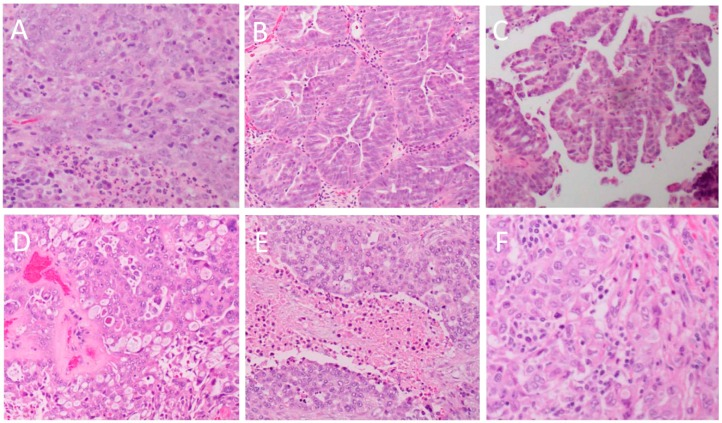
\includegraphics[width=\textwidth]{Introduction/Figs/Raster/ijms-20-00952-g001.jpg}
    \caption[Morphology types in HGSOC]{Heterogeneous morphology of HGSOC tissues, examples from Murakami \textit{et. al.}\citep{murakami2016establishment}. A) Solid growth architecture B) C) D) E). }
    \label{fig:morphology_murakami}
\end{figure}
\citep{murakami2016establishment, Lisio2019Feb}

\subsection{Collagen}
Collagen is the main component of the extracellular matrix, collagen deposition is a key part of desmoplasia. 
Experiments that assessed the expression of genes in both cisplatin resistant and sensitive OVC cells, many ECM genes were elevated in cisplatin-resistant cells. COL6A3 was one of the most highly upregulated genes, and cultivation of cisplatin-sensitive cells in the presence of collagen VI protein promoted resistance in vitro\cite{Sherman-Baust2003Apr}. Work by Januchowski et. al. in 2016 found similar results\cite{januchowski2016increased}. There is much evidence to suggest that collagen remodelling is utilized by cells to aid survival in the presence of chemotoxic drugs. Collagen remodelling has also been linked to increased motility and promotion of metastasis\cite{natarajan2019collagen}.

\subsection{Second-harmonic generation}

Second harmonic generation(SHG) is a nonlinear optical process in which two photons with the same frequency interact with a nonlinear material and combine to make a single new photon with twice the energy of the initial photons (half the wavelength). Collagen fibres are one such non-linear material and can be imaged using the SHG method. An advantage of this is that SHG imaging is marker free and so can be carried out without the requirement of antigen retrieval. 


%********************************** %Second Section  *************************************
\section{What drives HGSOC?} %Section - 1.2

TP53 mutations are believed to be ubiquitous in high grade serous. The HGSOC genome is extremely complex and highly rearranged. In the face of such complexity it is difficult to elucidate exactly what is causing what.  \citep{RN17}


\nomenclature[z-HGSOC]{HGSOC}{High Grade Serous Ovarian Cancer}
\nomenclature[z-TMA]{TMA}{Tissue Micro Array}
\nomenclature[z-IMC]{IMC}{Immuno Metal Conjugation}
\nomenclature[z-IHC]{IHC}{Immuno histo chemistry}
\nomenclature[z-IF]{IF}{Immunofluorescence}
\nomenclature[z-SHG]{SHG}{Second Harmonic Generation}
\nomenclature[z-GLCM]{GLCM}{Grey Level Co-occurence Matrix}

